%
The following code plots Fig. \ref{fig:3.8.6_triangle1}
\begin{lstlisting}
solutions/6/codes/line/motion_plane/man_river.py
\end{lstlisting}  
\begin{figure}[!ht]
\centering
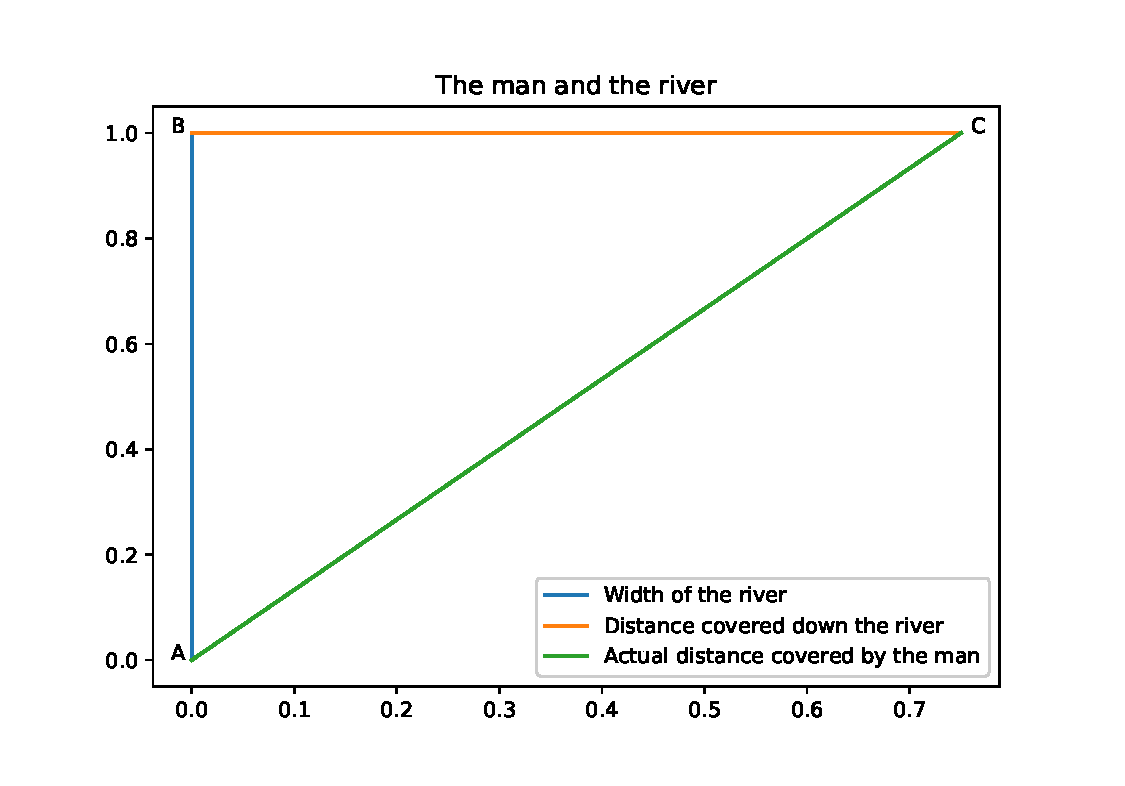
\includegraphics[width=\columnwidth]{./solutions/6/codes/line/motion_plane/man_river.eps}
\caption{}
\label{fig:3.8.6_triangle1}
\end{figure}
In Fig. \ref{fig:3.8.6_triangle1}, let the man be at
\begin{align}
\vec{A} = \myvec{0\\0}
\end{align}
The opposite bank of the river is at 
\begin{align}
\vec{B} = \myvec{1\\0}
\end{align}
River current
\begin{align}
\vec{v} = \myvec{3\\0}
\end{align}
Initial velocity of the man  is
\begin{align}
\vec{u} = \myvec{0\\4}
\end{align}
%
The resultant velocity of the man is 
\begin{align}
\vec{u}+\vec{v} = \myvec{3\\4}
\end{align}
If the time taken by the man to cross the river be t, then
\begin{align}
\vec{C} &= \brak{\vec{u}+\vec{v}}t = \myvec{3\\4}t
\\
&= \vec{A}+\vec{B}  = \myvec{BC\\1}
\end{align}
%
Thus,
\begin{align}
\myvec{3\\4}t &=  \myvec{BC\\1}
\\
\implies 4t = 1 \text{or, } t &= \frac{1}{4}
\end{align}
Distance traveled down the river
%
\begin{align}
BC = 3t = \frac{3}{4}
\end{align}
%

